











\begin{figure*}[h]
\centering
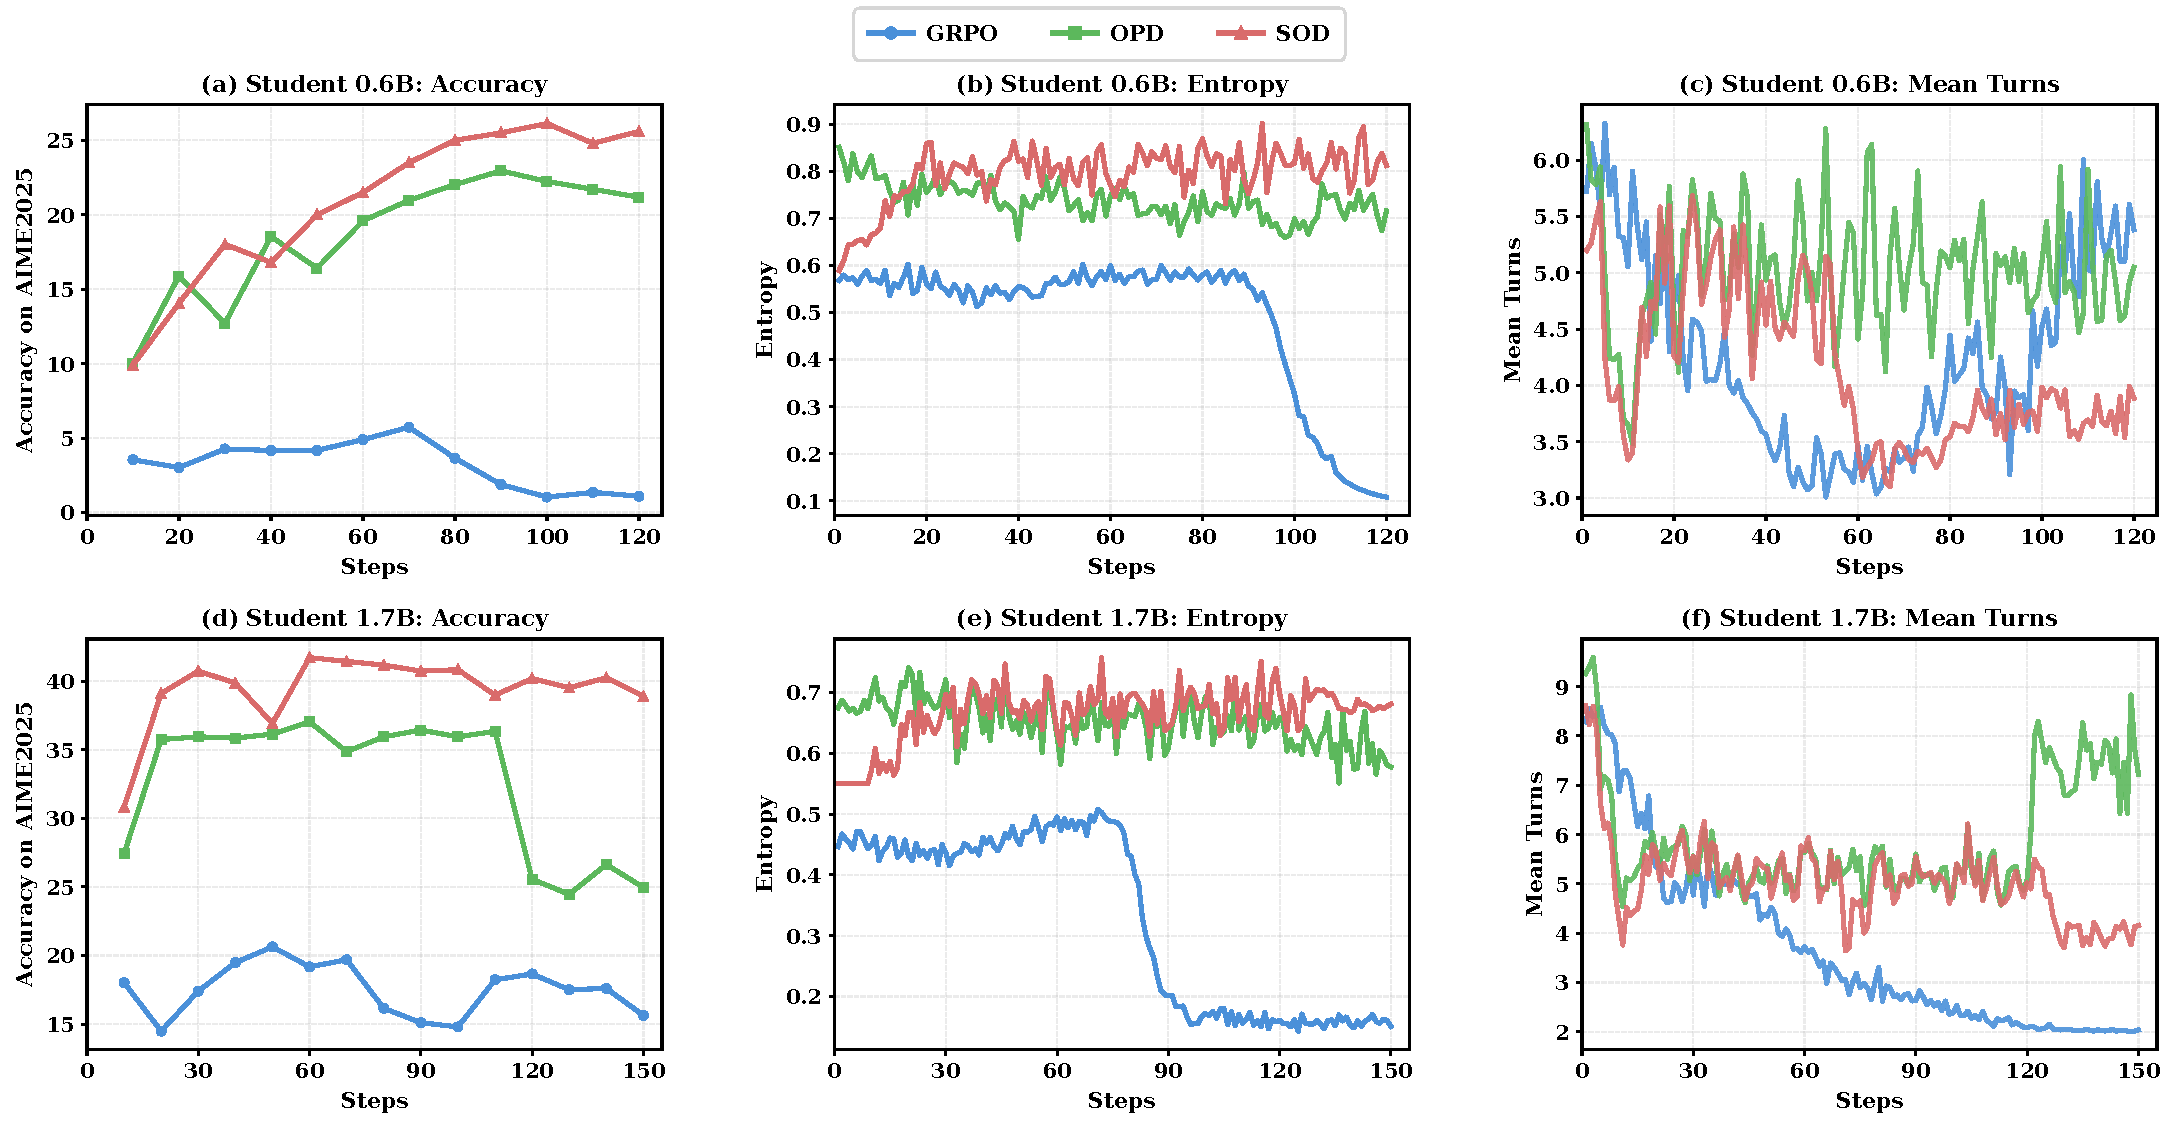
\includegraphics[width=1.0\linewidth]{pic/rq4_combined_2x3_v6.pdf}
\caption{\textbf{Training dynamics across methods on 0.6B and 1.7B student models}. We track accuracy on AIME2025 (left), policy entropy (middle), and mean tool-calling turns (right) throughout training.}
\label{rq4}
\end{figure*}



\subsection{Dynamic training analysis}


To understand how \ourmodel shapes the learning dynamics of agentic reasoning, we monitor three key metrics throughout training: task accuracy, policy entropy, and mean tool-calling turns. As shown in Figure~\ref{rq4}, we highlight the following observations:




\begin{itemize}[leftmargin=*]

\item \textbf{Obs 6: \ourmodel consistently outperforms GRPO by a large margin.} As shown in Figure~\ref{rq4}(a)(d), \ourmodel achieves significantly higher accuracy than GRPO across both model scales. This gap is driven by GRPO's severe entropy collapse (Figure~\ref{rq4}(b)(e)), where the policy loses exploration ability and degenerates into repetitive outputs, ultimately abandoning multi-step tool interactions entirely (Figure~\ref{rq4}(c)(f)), a fatal failure mode for TIR tasks.












\item \textbf{Obs 7: \ourmodel achieves more stable training than OPD.} 
While OPD maintains comparable entropy levels, its accuracy exhibits notable instability, particularly on 1.7B where performance peaks early then degrades significantly (Figure~\ref{rq4}(d)), suggesting that uniform distillation can destabilize later training. 
In contrast, \ourmodel sustains steady improvement without degradation. Additionally, \ourmodel uses fewer tool-calling turns than OPD (Figure~\ref{rq4}(c)(f)), indicating more efficient reasoning with fewer erroneous intermediate steps.

\end{itemize}



